\chapter{Preprocessing}

Quella che sarà descritta in questo capitolo è sicuramente la fase più impegnativa e delicata. Vista quindi l'importanza che l'attività di preprocessing ha rivestito nella riuscita dell'intero lavoro, è stato scelto di descriverla con un elevato livello di dettaglio, evidenziando passaggio per passaggio le varie operazioni svolte per trasformare la forma dell'insieme di dati grezzi in una adeguata al tipo di analisi che ci si è prefissati di fare. \\

Nell'illustrare le varie operazioni svolte, per favorire una spiegazione lineare e il più possibile comprensibile, si impiegherà talvolta la metafora della lavorazione meccanica, intesa in questo caso come una sgrossatura volta ad ottenere un semilavorato --- il data set \textit{preprocessato}, pronto per essere ulteriormente lavorato con le tecniche di \textit{data mining}. Ricordando quanto affermato l'introduzione della sezioni precedenti, i dati iniziali rappresentano il pezzo grezzo da lavorare, e le tecnologie scelte gli utensili da impiegare nella sgrossatura.

\section{Preparazione dell'Ambiente di Lavoro}

	\subsection{Ottenere gli strumenti necessari}

		Innanzitutto, è necessario predisporre gli utensili necessari al lavoro da svolgere --- fuor di metafora, si tratta di installare i programmi necessari al \textit{preprocessing}. Come abbiamo detto nella sezione dedicata alla \textit{technology stack}, abbiamo bisogno del \textit{d.b.m.s.} MongoDB e del suo \textit{driver}\footnote{il termine \textit{driver} non è perfettamente proprio per descrivere quella che in realtà è una semplice implementazione in Python delle \textit{A.P.I.} di MongoDB, ma colloquialmente rende bene l'idea della funzione di \texttt{pymongo}.}.

		La piattaforma impiegata è un personal computer con sistema operativo Arch Linux, perciò occorrerà installare MongoDB su di essa. Questo può essere fatto in modo estremamente agile, scaricando i pacchetti \texttt{mongodb} e \texttt{mongodb-tools} dalle repository ufficiali con il seguente comando:

		\begin{lstlisting}[language=bash,caption={installazione di MongoDB}]
			sudo pacman -S mongodb mongodb-tools --noconfirm
		\end{lstlisting}

		Per ottenere \texttt{pymongo}, invece, occorre utilizzare il \textit{package manager} di Python, \texttt{pip}, invocandolo semplicemente come segue:

		\begin{lstlisting}[language=bash,caption={installazione di pymongo}]
			pip install pymongo
		\end{lstlisting}

		A questo punto disponiamo degli utensili necessari per la nostra lavorazione.

	\subsection{Inizializzazione di un server MongoDB}

	Occorre adesso avviare la macchina e montare il pezzo --- in una \textit{vera} lavorazione meccanica, ovviamente \textit{prima} si monta l'utensile e si posiziona il pezzo, \textit{poi} si avvia la macchina; in questo caso occorre avviare prima un processo di MongoDB affinché si possano importare i dati grezzi in uno \textit{schema} ed organizzarli in \textit{collections}, per poi lavorarli tramite \texttt{pymongo}. \\

	MongoDB fornisce un database estremamente veloce, e di default utilizza come supporto fisico di memorizzazione una cartella sul disco di installazione. La macchina utilizzata dispone di un disco a stato solido come supporto di memoria non volatile, perciò le velocità di lettura e scrittura nel database di MongoDB risulterebbero ottime anche nella configurazione standard. Tuttavia, sia per migliorare ulteriormente le performances delle operazioni che per preservare la vita del disco\footnote{le celle di memoria degli SSD, o dischi a stato solido, possono sopportare un numero limitato di scritture prima di rovinarsi.}, è stato scelto di creare un \textit{ramdisk}\footnote{\textit{filesystem} implementato in un'area di RAM; è una tecnica per velocizzare estremamente le operazioni di lettura e scrittura, ma dato che il \textit{filesystem} è implementato su memoria volatile, i dati scritti in esso vengono persi dopo lo spegnimento della macchina.} da far utilizzare a MongoDB come supporto fisico di memoria. \\

	Per pura comodità, le operazioni necessarie per realizzare quanto appena descritto sono state delegate ad uno script:

		\begin{lstlisting}[language=bash,caption={script di lancio di un server MongoDB}, numbers=left, stepnumber=1]
			#!/bin/zsh
			sudo killall mongod
			yes | rm -rf /mnt/ramdisk/db
			mkdir db /mnt/ramdisk/db
			mongod --dbpath=/mnt/ramdisk/db
		\end{lstlisting}

	Nella \textit{shell} con cui è stato lanciato questo script si può vedere lo \textit{standard output} del processo \texttt{mongod}. Significa che MongoDB è attivo ed invocabile tramite gli strumenti a nostra disposizione.

	\subsection{Importazione dei Dati Grezzi}

	A questo punto, gli utensili sono pronti: occorre posizionare il pezzo grezzo da lavorare, ovvero importare i dati grezzi in MongoDB. \\

	Come visto nel capitolo precedente, i dati a disposizioni sono contenuti in sette file \texttt{csv}: si manterrà questa struttura --- almeno inizialmente --- importando quindi ogni file in una sua \textit{collection}. Come is può vedere di seguito, questa operazione è stata descritta nel \texttt{makefile} con l'etichetta \texttt{import}:

	\begin{center}
		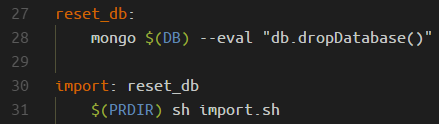
\includegraphics[scale=0.7]{img/import.png}
	\end{center}

	Le variabili \texttt{\$(DB)} e \texttt{\$(PRDIR)} sono specifiche dell'ambiente predisposto\footnote{per un esempio pratico, si consulti l'intero \texttt{makefile} riportato in \ref{appendix:makefile}.}. Essa si può lanciare con il seguente semplice comando di \texttt{shell}:

	\begin{lstlisting}[language=bash,caption={importazione dei dati in MongoDB}]
		make import
	\end{lstlisting}

	La vera e propria invocazione del comando necessario all'import dei file nel database --- \texttt{mongoimport}, del pacchetti \texttt{mongodb-tools} --- è stata delegata in un file esterno al \texttt{makefile}, per preservare la compattezza e la brevità di quest'ultimo. Si veda comunque di seguito il comando per l'import di uno dei sette file: 

	\begin{lstlisting}[language=bash,caption={dettaglio dell'importazione dei dati in MongoDB}]
		mongoimport -d exams -c rawStudentsPr1013 --type csv --file ../raw/prod_stud_10-11-12-13.csv --headerline
	\end{lstlisting}

	Il comando, come ogni chiamata da \texttt{shell}, ha degli argomenti che ne specificano il comportamento. In questo caso, sono:

	\begin{itemize}
		\item \texttt{-d}: il database nel quale importare i dati;
		\item \texttt{-c}: la collection nella quale inserire i dati;
		\item \texttt{-type}: il tipo del file da leggere;
		\item \texttt{-file}: il riferimento al file;
		\item \texttt{-headerline}: indica che gli attributi delle istanze sono specificati nella prima riga del file.
	\end{itemize}

	A questo punto, nel database \texttt{exams} di MongoDB ci sono otto \textit{collections}, contenenti i \textit{documenti} che rappresentano le istanze dei dati a disposizione.

\section{Aggregazione per Anno Accademico: dati degli studenti}

\section{Aggregazione per Anno Accademico: valutazioni dei corsi}

\section{Join dei due insiemi di dati con attributi continui}

\section{Join dei due insiemi di dati con attributi discreti}

\section{Sequenze ordinate di esami superati}

\section{Estrazione dei data set preprocessati}

	\begin{center}
		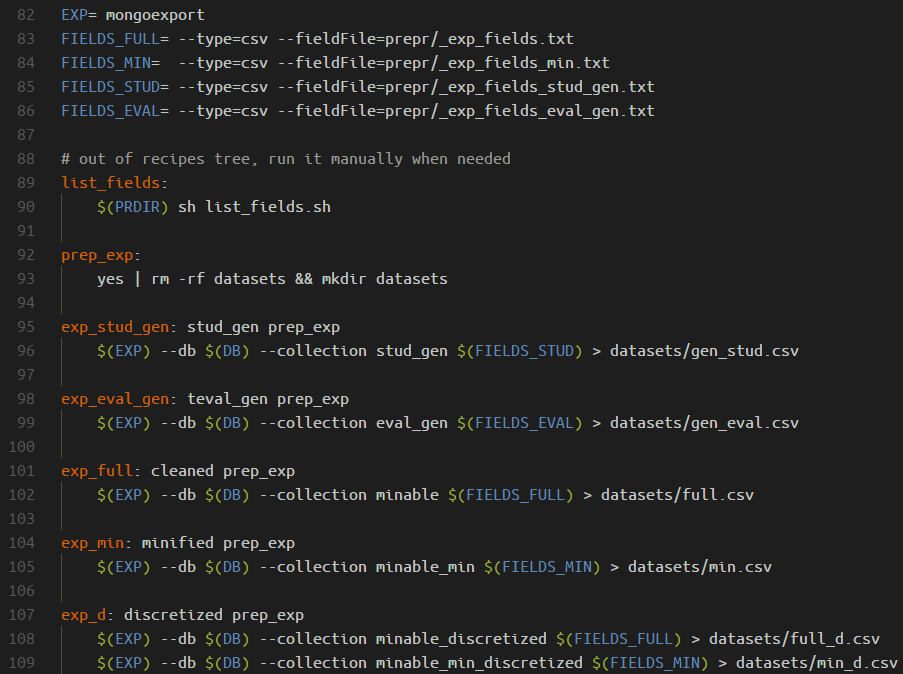
\includegraphics[scale=0.7]{img/export.png}
	\end{center}

	\lstinputlisting[language=bash,caption={script di shell per ottenere una lista degli attributi dei documenti in una collezione}, numbers=left, stepnumber=1]{../prepr/list_fields.sh}

	\lstdefinelanguage{JavaScript}{
  		keywords={break, case, catch, continue, debugger, default, delete, do, else, finally, for, function, if, in, instanceof, new, return, switch, this, throw, try, typeof, var, void, while, with},
 		morecomment=[l]{//},
  		morecomment=[s]{/*}{*/},
  		morestring=[b]',
  		morestring=[b]",
  		sensitive=true
	}

	\lstinputlisting[language=JavaScript,caption={script della shell di MongoDB per ottenere la lista degli attributi dei documenti in una collezione}, numbers=left, stepnumber=1]{../prepr/list_attr.mongosh}
